\chapter{Manual de instalación}
\label{chap:install}

Debido a que la herramienta se ha desarrollado en forma de una página web, para ponerla en funcionamiento únicamente hará falta instalar Ruby on Rails en el sistema anfitrión y lanzar el servidor que instala el entorno de programación, de esta manera podremos acceder al desarrollo desde nuestra máquina local.\\
Este manual está destinado a la instalación del lenguaje de programación Ruby on Rails, la descarga de la herramienta y su puesta en funcionamiento bajo el sistema operativo \textit{Elementary OS}.
\section{Herramienta Web}

\subsection{Instalación de Ruby on Rails}

Primero se prepara el sistema instalando los paquetes auxiliares necesarios para la descarga de Ruby, para lo cual se abre una terminal y se escriben los siguientes comandos:

\begin{console}
	$ sudo apt-get update
	$ sudo apt-get install build-essential git
\end{console}%$

A continuación se instala la firma necesaria para la descarga de RVM escribiendo en la terminal:

\begin{console}
	$ gpg --keyserver hkp://keys.gnupg.net --recv-keys 409B6B1796C275462A1703113804BB82D39DC0E3
\end{console}%$

Por último, para instalar las últimas versiones estables de RVM, Ruby y Rails se ejecuta la siguiente orden en el terminal:

\begin{console}
	$ \curl -sSL https://get.rvm.io | bash -s stable
\end{console}%$

Una vez instalado se reinicia la terminal y se lanza el siguiente comando para completar la instalación de Ruby en la versión 2.1.2:

\begin{console}
	$ rvm install ruby 2.1.2
\end{console}%$

Indicamos a RVM que esta es la versión de Ruby que usaremos por defecto:

\begin{console}
	$ rvm use 2.1.2 --default
\end{console}%$

El siguiente paso consiste en descargar e instalar Rails y un entorno de ejecución para JavaScript, en este caso NodeJS:

\begin{console}
	$ gem install rails
	$ sudo apt-get install nodejs
\end{console}%$

\subsection{Clonar repositorio herramienta e iniciar Rails}

Para descargar el código fuente desde el repositorio se debe clonar el repositorio de Github, ejecutar el administrador de gemas e iniciar el servidor Rails:

\begin{console}
	$ git clone https://github.com/jbausa/mementoParking_CODE.git
	$ cd mementoParking_CODE
	$ bundle install
	$ rails s
\end{console}%$

Una vez realizados estos pasos, se podrá abrir un navegador y acceder a la aplicación desde la dirección \url{http://localhost:3000}.

\section{Despliegue en Heroku}

La herramienta ha sido desplegada en un servidor externo, de manera que se puede acceder a la misma desde un navegador utilizando la dirección \url{http://mementoparking.herokuapp.com/}.

\section{Instalación de Android Studio}
Para la instalación de Android Studio se accede a la página oficial y se descarga el archivo continente del programa. Una vez descomprimido se podrá acceder mediante la terminal, desde la carpeta \textit{bin/} del programa ejecutando el comando \textit{./studio.sh}.

\section{Clonar repositorio Aplicación e iniciar Android}

Una vez dentro de la aplicación seleccionando la opción \textit{GitHub} dentro de \textit{Project from Version Control} en el menú \textit{New} (ver figura \ref{fig:android-studio}) y escribiendo la dirección del repositorio.

\begin{figure}[H]
\centering
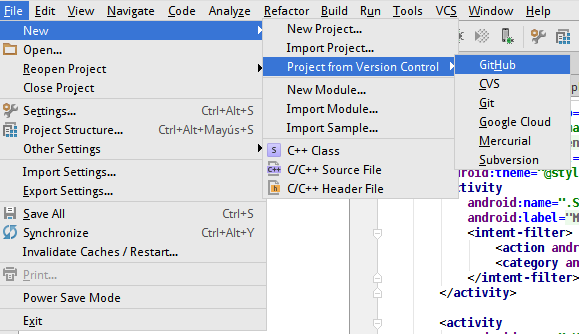
\includegraphics[scale=0.5, fbox={\fboxrule} 4mm]{images/07-anexo/01-android_studio.png}
\caption{Importar proyecto}
\label{fig:android-studio}
\end{figure}

Para lanzar la aplicación será necesario instalar previamente los SDK necesarios y configurar un dispositivo virtual sobre el que mostrarla.

\section{Archivo aplicación}
En el repositorio correspondiente se encuentra un archivo APK con la aplicación preparada para la instalación en los dispositivos compatibles.


% Local Variables:
%  coding: utf-8
%  mode: latex
%  mode: flyspell
%  ispell-local-dictionary: "castellano8"
% End: